\hypertarget{ui-file-for-menu-and-action-entries}{%
\section{Ui file for menu and action
entries}\label{ui-file-for-menu-and-action-entries}}

\hypertarget{ui-file-for-menu}{%
\subsection{Ui file for menu}\label{ui-file-for-menu}}

You might have thought that building menus is really bothersome. Yes,
the program was complicated and it needs lots of time to code it. The
situation is similar to building widgets. When we built widgets, using
ui file was a good way to avoid such complicated coding. The same goes
for menus.

The ui file for menus has interface, menu tags. The file starts and ends
with interface tag.

\begin{lstlisting}[language=XML]
<interface>
  <menu id="menubar">
  </menu>
</interface>
\end{lstlisting}

\passthrough{\lstinline!menu!} tag corresponds to GMenu object.
\passthrough{\lstinline!id!} attribute defines the name of the object.
It will be referred by GtkBuilder.

\begin{lstlisting}[language=XML]
<submenu>
  <attribute name="label">File</attribute>
    <item>
      <attribute name="label">New</attribute>
      <attribute name="action">win.new</attribute>
    </item>
</submenu>
\end{lstlisting}

\passthrough{\lstinline!item!} tag corresponds to item in GMenu which
has the same structure as GMenuItem. The item above has a label
attribute. Its value is ``New''. The item also has an action attribute
and its value is ``win.new''. ``win'' is a prefix and ``new'' is an
action name. \passthrough{\lstinline!submenu!} tag corresponds to both
GMenuItem and GMenu. The GMenuItem has a link to GMenu.

The ui file above can be described as follows.

\begin{lstlisting}[language=XML]
<item>
  <attribute name="label">File</attribute>
    <link name="submenu">
      <item>
        <attribute name="label">New</attribute>
        <attribute name="action">win.new</attribute>
      </item>
    </link>
</item>
\end{lstlisting}

\passthrough{\lstinline!link!} tag expresses the link to submenu. And at
the same time it also expresses the submenu itself. This file
illustrates the relationship between the menus and items better than the
prior ui file. But \passthrough{\lstinline!submenu!} tag is simple and
easy to understand. So, we usually prefer the former ui file style.

The following is a screenshot of the sample program in this section. Its
name is \passthrough{\lstinline!menu3!}.

\begin{figure}
\centering
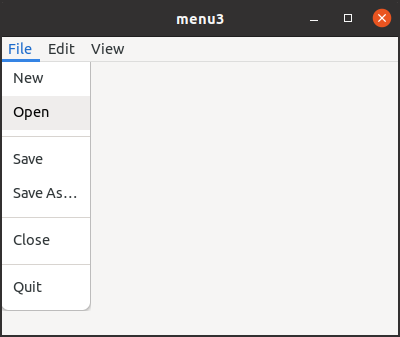
\includegraphics[width=6cm,height=5.055cm]{../image/menu3.png}
\caption{menu3}
\end{figure}

The following is the ui file of the menu in
\passthrough{\lstinline!menu3!}.

\begin{lstlisting}[language=XML, numbers=left]
<?xml version="1.0" encoding="UTF-8"?>
<interface>
  <menu id="menubar">
    <submenu>
      <attribute name="label">File</attribute>
      <section>
        <item>
          <attribute name="label">New</attribute>
          <attribute name="action">win.new</attribute>
        </item>
        <item>
          <attribute name="label">Open</attribute>
          <attribute name="action">win.open</attribute>
        </item>
      </section>
      <section>
        <item>
          <attribute name="label">Save</attribute>
          <attribute name="action">win.save</attribute>
        </item>
        <item>
          <attribute name="label">Save As…</attribute>
          <attribute name="action">win.saveas</attribute>
        </item>
      </section>
      <section>
        <item>
          <attribute name="label">Close</attribute>
          <attribute name="action">win.close</attribute>
        </item>
      </section>
      <section>
        <item>
          <attribute name="label">Quit</attribute>
          <attribute name="action">app.quit</attribute>
        </item>
      </section>
    </submenu>
    <submenu>
      <attribute name="label">Edit</attribute>
      <section>
        <item>
          <attribute name="label">Cut</attribute>
          <attribute name="action">win.cut</attribute>
        </item>
        <item>
          <attribute name="label">Copy</attribute>
          <attribute name="action">win.copy</attribute>
        </item>
        <item>
          <attribute name="label">Paste</attribute>
          <attribute name="action">win.paste</attribute>
        </item>
      </section>
      <section>
        <item>
          <attribute name="label">Select All</attribute>
          <attribute name="action">win.selectall</attribute>
        </item>
      </section>
    </submenu>
    <submenu>
      <attribute name="label">View</attribute>
      <section>
        <item>
          <attribute name="label">Full Screen</attribute>
          <attribute name="action">win.fullscreen</attribute>
        </item>
      </section>
    </submenu>
  </menu>
</interface>
\end{lstlisting}

The ui file is converted to the resource by the resource compiler
\passthrough{\lstinline!glib-compile-resouces!} with xml file below.

\begin{lstlisting}[language=XML, numbers=left]
<?xml version="1.0" encoding="UTF-8"?>
<gresources>
  <gresource prefix="/com/github/ToshioCP/menu3">
    <file>menu3.ui</file>
  </gresource>
</gresources>
\end{lstlisting}

GtkBuilder builds menus from the resource.

\begin{lstlisting}[language=C]
GtkBuilder *builder = gtk_builder_new_from_resource ("/com/github/ToshioCP/menu3/menu3.ui");
GMenuModel *menubar = G_MENU_MODEL (gtk_builder_get_object (builder, "menubar"));

gtk_application_set_menubar (GTK_APPLICATION (app), menubar);
g_object_unref (builder);
\end{lstlisting}

It is important that \passthrough{\lstinline!builder!} is unreferred
after the GMenuModel \passthrough{\lstinline!menubar!} is inserted to
the application. If you do it before setting, bad thing will happen --
your computer might freeze.

\hypertarget{action-entry}{%
\subsection{Action entry}\label{action-entry}}

The coding for building actions and signal handlers is bothersome work
as well. Therefore, it should be automated. You can implement them
easily with GActionEntry structure and
\passthrough{\lstinline!g\_action\_map\_add\_action\_entries!} function.

GActionEntry contains action name, signal handlers, parameter and state.

\begin{lstlisting}[language=C]
typedef struct _GActionEntry GActionEntry;

struct _GActionEntry
{
  /* action name */
  const gchar *name;
  /* activate handler */
  void (* activate) (GSimpleAction *action, GVariant *parameter, gpointer user_data);
  /* the type of the parameter given as a single GVariant type string */
  const gchar *parameter_type;
  /* initial state given in GVariant text format */
  const gchar *state;
  /* change-state handler */
  void (* change_state) (GSimpleAction *action, GVariant *value, gpointer user_data);
  /*< private >*/
  gsize padding[3];
};
\end{lstlisting}

For example, the actions in the previous section are:

\begin{lstlisting}[language=C]
{ "fullscreen", NULL, NULL, "false", fullscreen_changed }
{ "color", color_activated, "s", "red", NULL }
{ "quit", quit_activated, NULL, NULL, NULL },
\end{lstlisting}

And \passthrough{\lstinline!g\_action\_map\_add\_action\_entries!} does
all the process instead of the functions you have needed.

\begin{lstlisting}[language=C]
const GActionEntry app_entries[] = {
  { "quit", quit_activated, NULL, NULL, NULL }
};
g_action_map_add_action_entries (G_ACTION_MAP (app), app_entries,
                                 G_N_ELEMENTS (app_entries), app);
\end{lstlisting}

The code above does:

\begin{itemize}
\tightlist
\item
  Builds the ``quit'' action
\item
  Connects the action and the ``activate'' signal handler
  \passthrough{\lstinline!quit\_activated!}
\item
  Adds the action to the action map \passthrough{\lstinline!app!}.
\end{itemize}

The same goes for the other actions.

\begin{lstlisting}[language=C]
const GActionEntry win_entries[] = {
  { "fullscreen", NULL, NULL, "false", fullscreen_changed },
  { "color", color_activated, "s", "red", NULL }
};
g_action_map_add_action_entries (G_ACTION_MAP (win), win_entries,
                                 G_N_ELEMENTS (win_entries), win);
\end{lstlisting}

The code above does:

\begin{itemize}
\tightlist
\item
  Builds a ``fullscreen'' action and ``color'' action.
\item
  Connects the ``fullscreen'' action and the ``change-state'' signal
  handler \passthrough{\lstinline!fullscreen\_changed!}
\item
  Its initial state is set to FALSE.
\item
  Connects the ``color'' action and the ``activate'' signal handler
  \passthrough{\lstinline!color\_activated!}
\item
  Its parameter type is string and the initial value is ``red''.
\item
  Adds the actions to the action map \passthrough{\lstinline!win!}.
\end{itemize}

\hypertarget{example-code}{%
\subsection{Example code}\label{example-code}}

The C source code of \passthrough{\lstinline!menu3!} and
\passthrough{\lstinline!meson.build!} is as follows.

\begin{lstlisting}[language=C, numbers=left]
#include <gtk/gtk.h>

static void
new_activated (GSimpleAction *action, GVariant *parameter, gpointer win) {
}

static void
open_activated (GSimpleAction *action, GVariant *parameter, gpointer win) {
}

static void
save_activated (GSimpleAction *action, GVariant *parameter, gpointer win) {
}

static void
saveas_activated (GSimpleAction *action, GVariant *parameter, gpointer win) {
}

static void
close_activated (GSimpleAction *action, GVariant *parameter, gpointer win) {
}

static void
cut_activated (GSimpleAction *action, GVariant *parameter, gpointer win) {
}

static void
copy_activated (GSimpleAction *action, GVariant *parameter, gpointer win) {
}

static void
paste_activated (GSimpleAction *action, GVariant *parameter, gpointer win) {
}

static void
selectall_activated (GSimpleAction *action, GVariant *parameter, gpointer win) {
}

static void
fullscreen_changed (GSimpleAction *action, GVariant *state, gpointer win) {
  if (g_variant_get_boolean (state))
    gtk_window_maximize (GTK_WINDOW (win));
  else
    gtk_window_unmaximize (GTK_WINDOW (win));
  g_simple_action_set_state (action, state);
}

static void
quit_activated (GSimpleAction *action, GVariant *parameter, gpointer app)
{
  g_application_quit (G_APPLICATION(app));
}

static void
app_activate (GApplication *app, gpointer user_data) {
  GtkWidget *win = gtk_application_window_new (GTK_APPLICATION (app));

  const GActionEntry win_entries[] = {
    { "new", new_activated, NULL, NULL, NULL },
    { "open", open_activated, NULL, NULL, NULL },
    { "save", save_activated, NULL, NULL, NULL },
    { "saveas", saveas_activated, NULL, NULL, NULL },
    { "close", close_activated, NULL, NULL, NULL },
    { "cut", cut_activated, NULL, NULL, NULL },
    { "copy", copy_activated, NULL, NULL, NULL },
    { "paste", paste_activated, NULL, NULL, NULL },
    { "selectall", selectall_activated, NULL, NULL, NULL },
    { "fullscreen", NULL, NULL, "false", fullscreen_changed }
  };
  g_action_map_add_action_entries (G_ACTION_MAP (win), win_entries, G_N_ELEMENTS (win_entries), win);

  gtk_application_window_set_show_menubar (GTK_APPLICATION_WINDOW (win), TRUE);

  gtk_window_set_title (GTK_WINDOW (win), "menu3");
  gtk_window_set_default_size (GTK_WINDOW (win), 400, 300);
  gtk_widget_show (win);
}

static void
app_startup (GApplication *app, gpointer user_data) {
  GtkBuilder *builder = gtk_builder_new_from_resource ("/com/github/ToshioCP/menu3/menu3.ui");
  GMenuModel *menubar = G_MENU_MODEL (gtk_builder_get_object (builder, "menubar"));

  gtk_application_set_menubar (GTK_APPLICATION (app), menubar);
  g_object_unref (builder);

  const GActionEntry app_entries[] = {
    { "quit", quit_activated, NULL, NULL, NULL }
  };
  g_action_map_add_action_entries (G_ACTION_MAP (app), app_entries, G_N_ELEMENTS (app_entries), app);
}

#define APPLICATION_ID "com.github.ToshioCP.menu3"

int
main (int argc, char **argv) {
  GtkApplication *app;
  int stat;

  app = gtk_application_new (APPLICATION_ID, G_APPLICATION_FLAGS_NONE);
  g_signal_connect (app, "startup", G_CALLBACK (app_startup), NULL);
  g_signal_connect (app, "activate", G_CALLBACK (app_activate), NULL);

  stat =g_application_run (G_APPLICATION (app), argc, argv);
  g_object_unref (app);
  return stat;
}
\end{lstlisting}

meson.build

\begin{lstlisting}[numbers=left]
project('menu3', 'c')

gtkdep = dependency('gtk4')

gnome=import('gnome')
resources = gnome.compile_resources('resources','menu3.gresource.xml')

sourcefiles=files('menu3.c')

executable('menu3', sourcefiles, resources, dependencies: gtkdep)
\end{lstlisting}
